 
\vspace{-6mm}\begin{center}
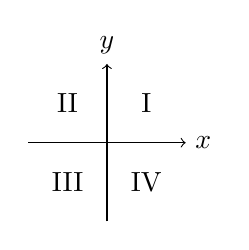
\begin{tikzpicture}[scale=0.5]
\draw[->](-2,0)--(2,0)node[anchor=west]{$x$};
\draw[->](0,-2)--(0,2)node[anchor=south]{$y$};
\draw(1,1)node{I}(-1,1)node{II}(-1,-1)node{III}(1,-1)node{IV};
\end{tikzpicture}
\end{center}
If the system of inequalities $y>x^2-4$ and $y \leq 2x-1$, which quadrant contains no solutions to the system?


\ifsat
	\begin{enumerate}[label=\Alph*)]
		\item Quadrant IV
		\item Quadrant II % 
		\item Quadrant I
		\item There are solutions in all four quadrants.
	\end{enumerate}
\else
\fi

\ifacteven
	\begin{enumerate}[label=\textbf{\Alph*.},itemsep=\fill,align=left]
		\setcounter{enumii}{5}
		\item Quadrant IV
		\item Quadrant II % 
		\item Quadrant I
		\addtocounter{enumii}{1}
		\item There are solutions in all four quadrants.
		\item None of these. 
	\end{enumerate}
\else
\fi

\ifactodd
	\begin{enumerate}[label=\textbf{\Alph*.},itemsep=\fill,align=left]
		\item Quadrant IV
		\item Quadrant II % 
		\item Quadrant I
		\item There are solutions in all four quadrants.
		\item None of these. 
	\end{enumerate}
\else
\fi

\ifgridin
 Quadrant II % 
		
\else
\fi

